\section{Размерная структура {\it Macoma balthica} в исследованных поселениях Баренцева моря} 
\label{app:Barents_sizestr_hist}
На всех графиках абсцисса --- длина раковины, мм; ордината --- численность особей, экз./м$^2$. Указано средняя численность особей определенного размера $\pm$ ошибка средней.
%%%%%%%%%%%%%%%%%%%%%%%%%%%%%%%%%%%%%
%Баренцево море

	\begin{figure}[hp]
	
	\begin{minipage}[b]{.46\linewidth}
	\begin{center}
	{\footnotesize Абрам-мыс, СГЛ}
		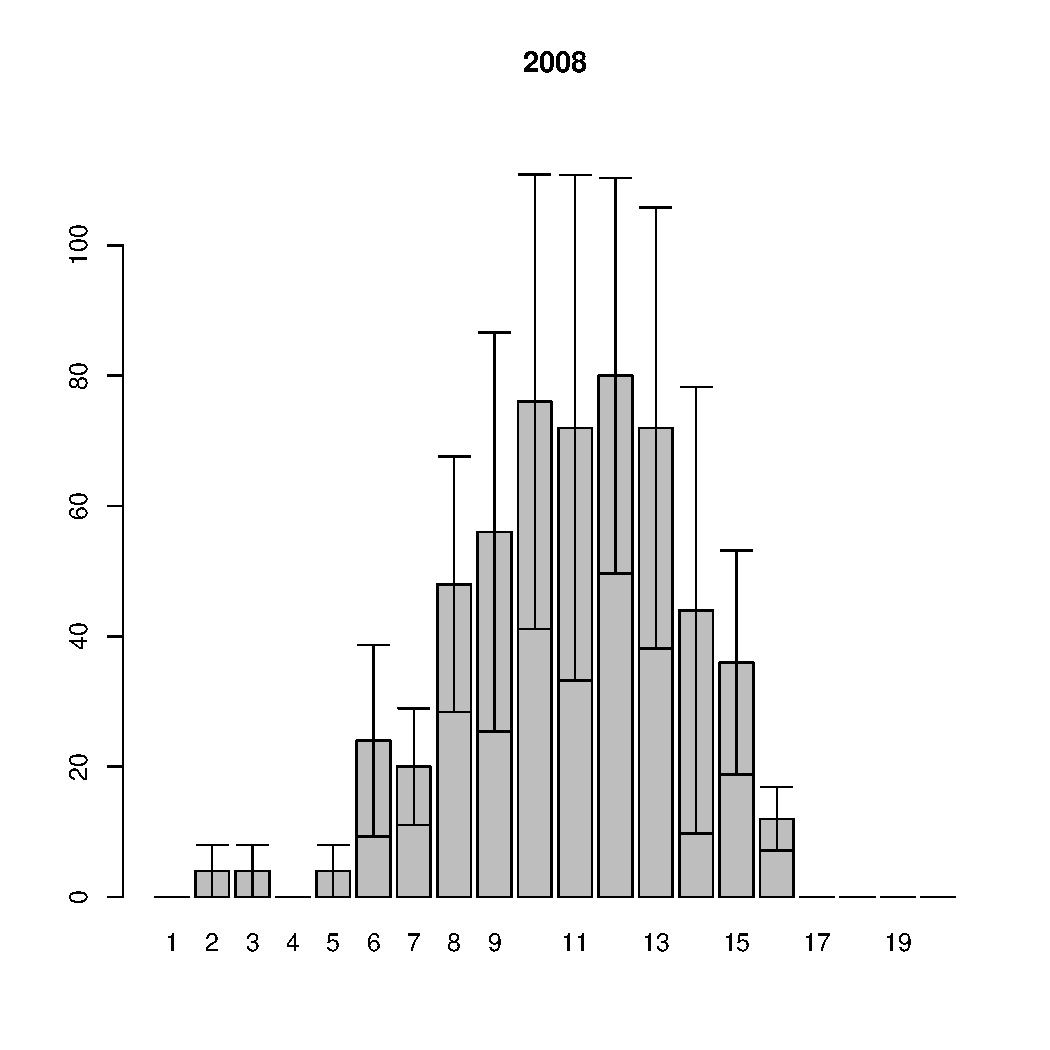
\includegraphics[width=55mm]{../Barenc_Sea/Abram-mys/middle_2008_.pdf}
	\end{center}
	\end{minipage}
	%
	\hfil %Это пружинка отодвигающая рисунки друг от друга
	%
	\begin{minipage}[b]{.46\linewidth}
	\begin{center}
	{\footnotesize Абрам-мыс, НГЛ}
		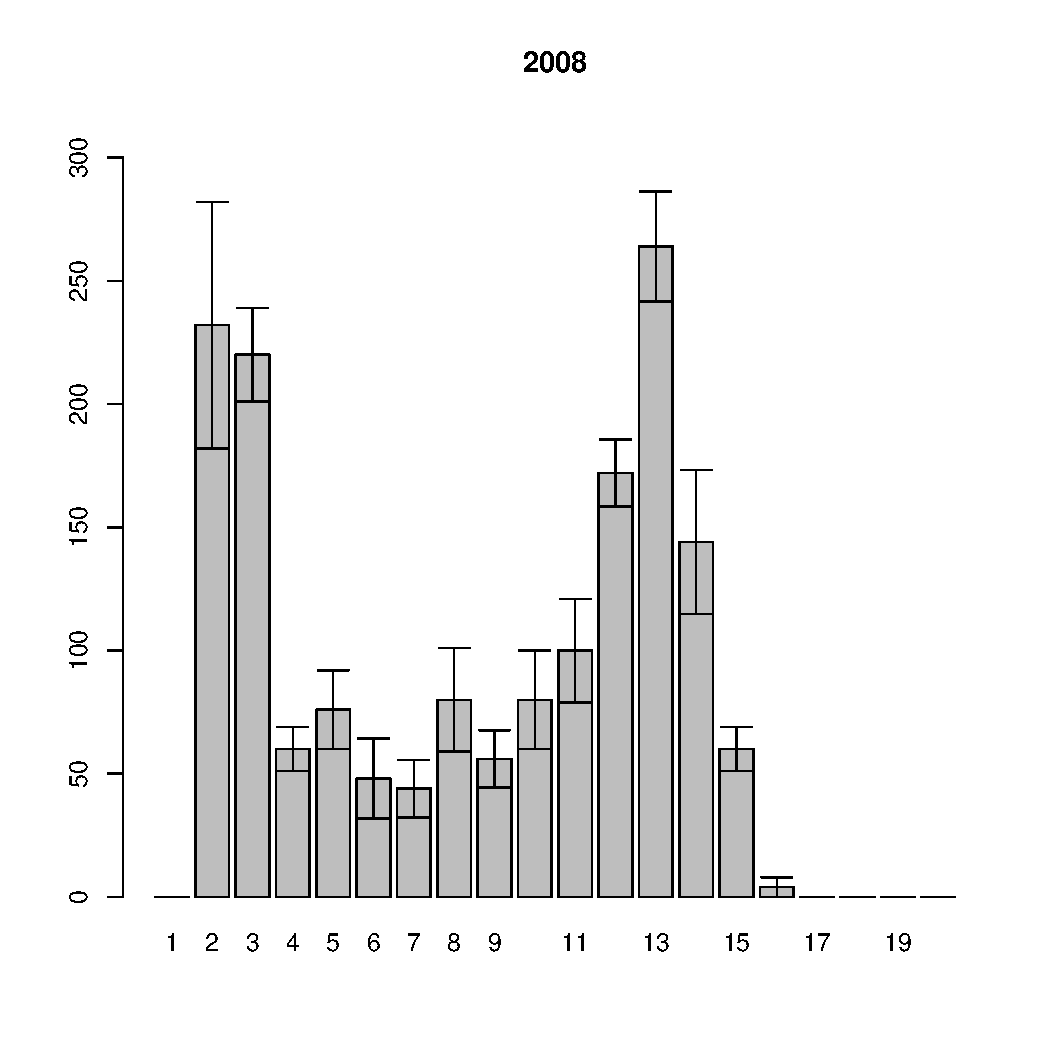
\includegraphics[width=55mm]{../Barenc_Sea/Abram-mys/low_2008_.pdf}
	\end{center}
	\end{minipage}
	%\smallskip
	\begin{minipage}[b]{.46\linewidth}
	\begin{center}
	{\footnotesize Пала-губа, СГЛ}
	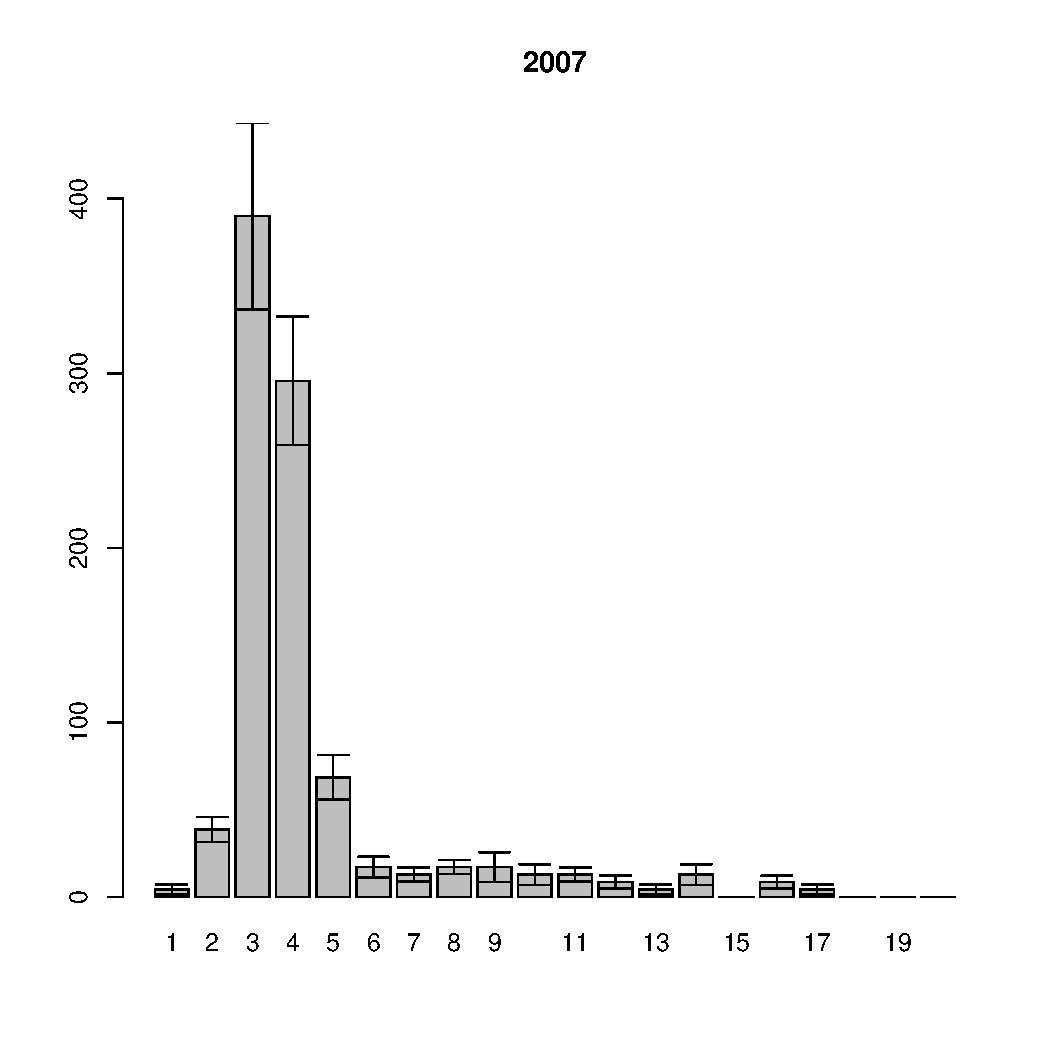
\includegraphics[width=55mm]{../Barenc_Sea/Pala/middle_2007_.pdf}
	\end{center}
	\end{minipage}
	%	
	\hfil %Это пружинка отодвигающая рисунки друг от друга
	%
	\begin{minipage}[b]{.46\linewidth}
	\begin{center}	
	{\footnotesize Пала-губа, НГЛ}
	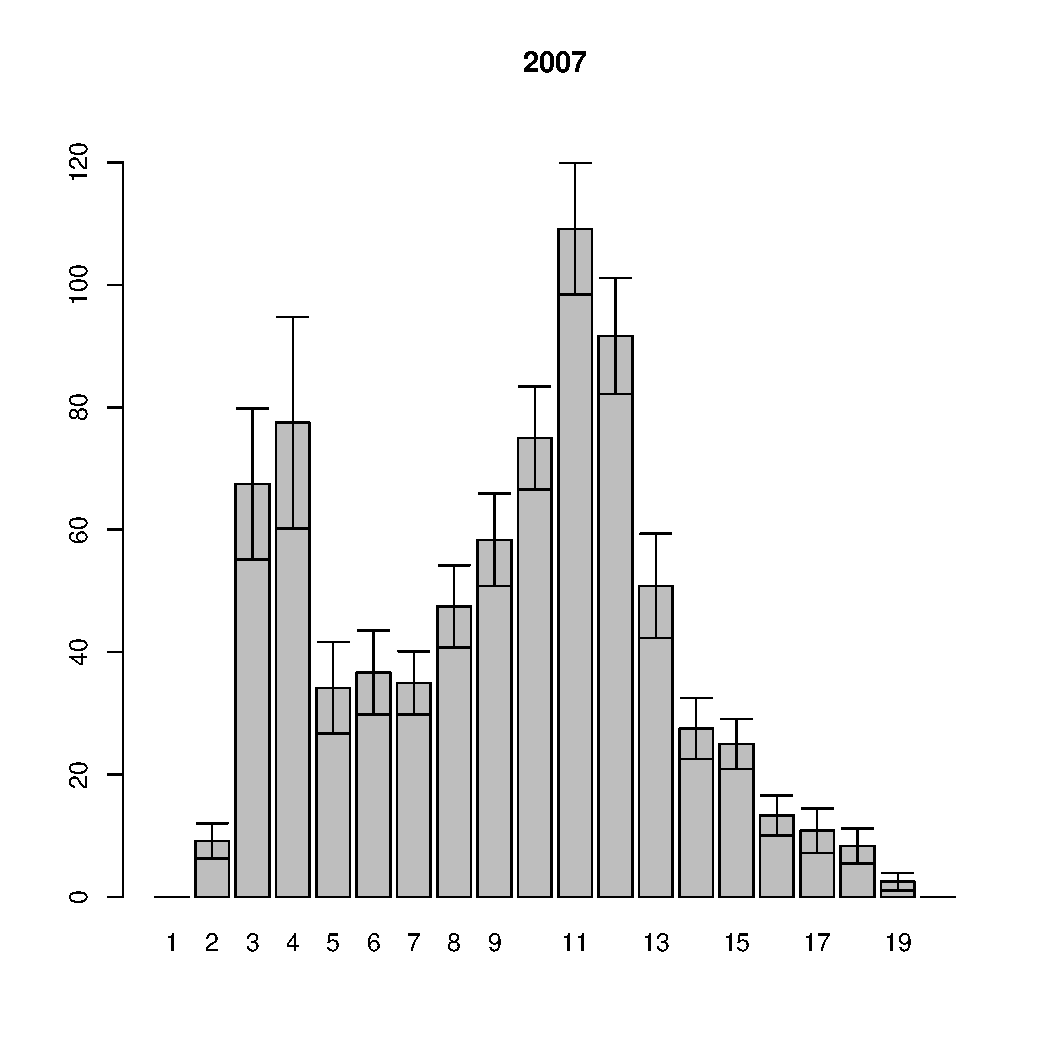
\includegraphics[width=55mm]{../Barenc_Sea/Pala/low_2007_.pdf}
	\end{center}
	\end{minipage}
	%\smallskip
	\begin{minipage}[b]{.46\linewidth}
	\begin{center}
	{\footnotesize Гаврилово, СГЛ}
	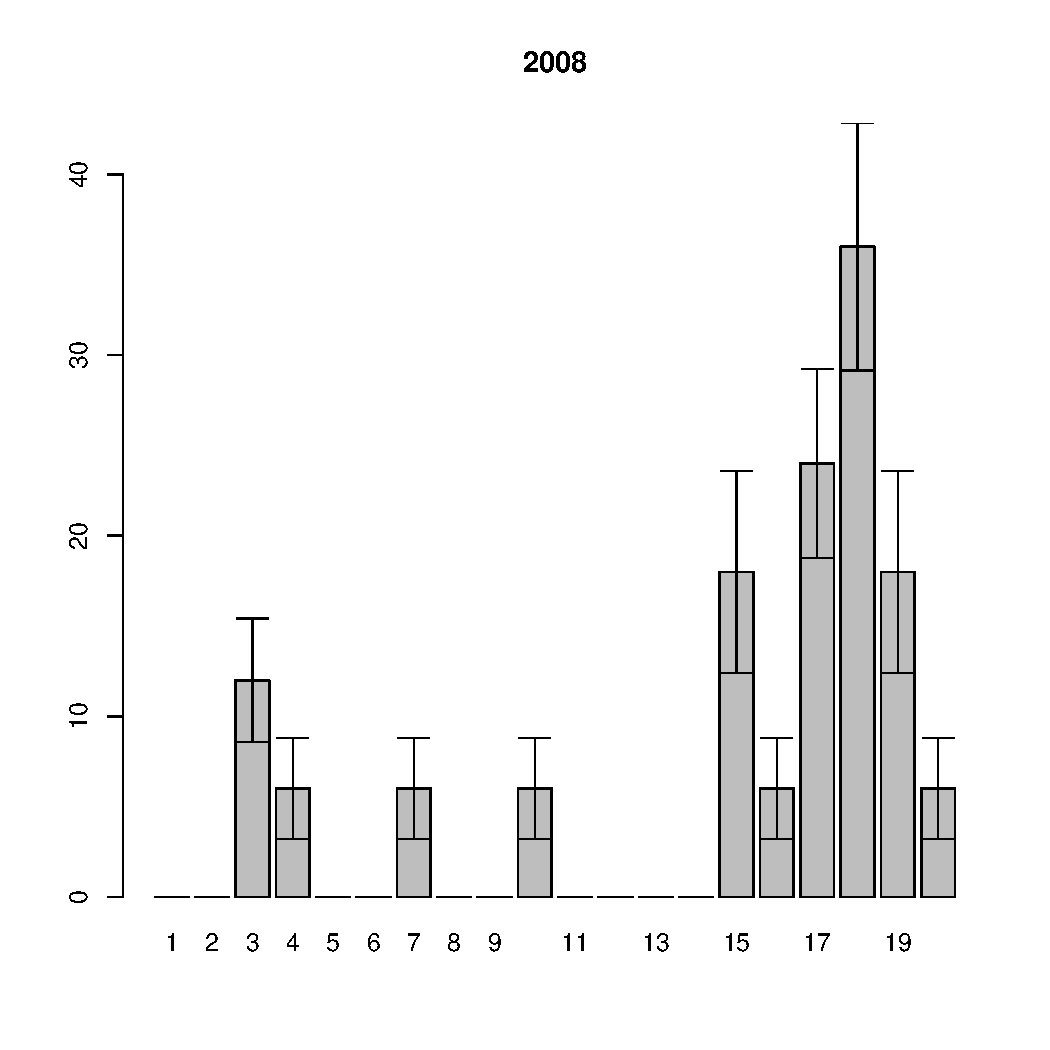
\includegraphics[width=55mm]{../Barenc_Sea/Gavrilovo/middle_2008_.pdf}
	\end{center}
	\end{minipage}
	%
	\hfil %Это пружинка отодвигающая рисунки друг от друга
	%
	\begin{minipage}[b]{.46\linewidth}
	\begin{center}
	{\footnotesize Порчниха, СГЛ}
	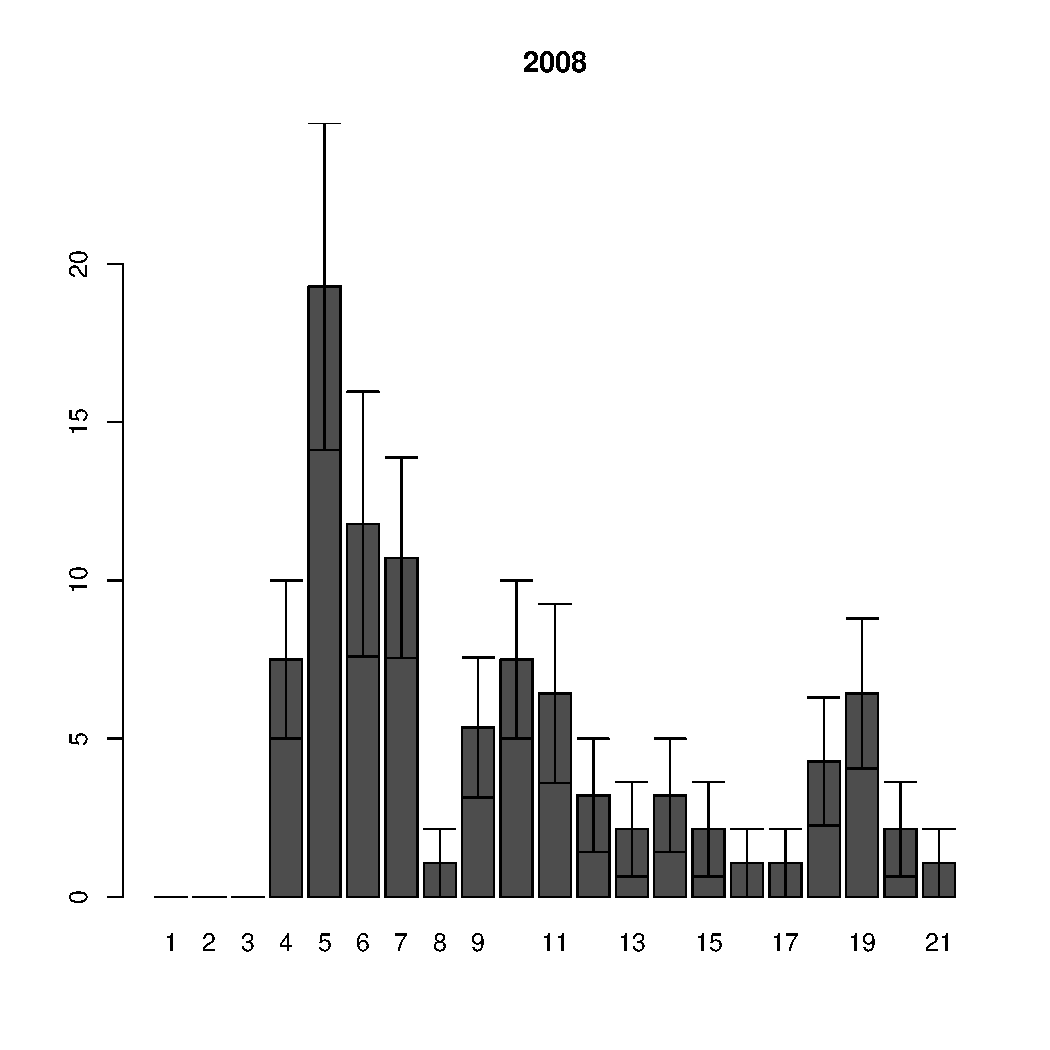
\includegraphics[width=55mm]{../Barenc_Sea/Porchnikha/sizestr2007.pdf}
	\end{center}
	\end{minipage}
	%\smallskip
\caption{Размерная структура {\it Macoma balthica} в поселениях Мурманского побережья Баренцева моря}
\label{ris:Barents_sizestr}
\end{figure}


%страница 2
	\begin{figure}[h]
	
	\begin{minipage}[b]{.46\linewidth}
	\begin{center}
	{\footnotesize Ярнышная, ВГЛ}
	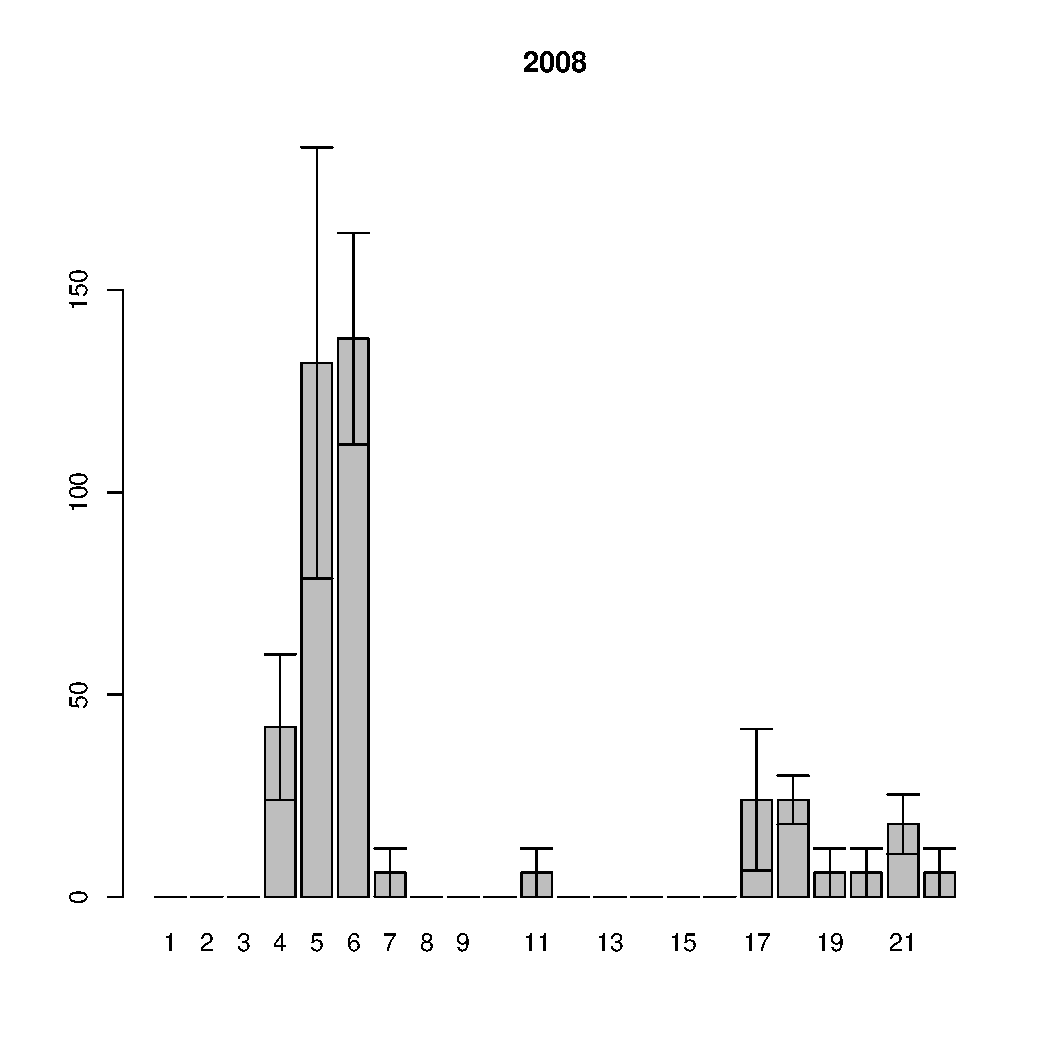
\includegraphics[width=55mm]{../Barenc_Sea/Yarnyshnaya/high_2008_.pdf}
	\end{center}
	\end{minipage}
	%
	\hfil %Это пружинка отодвигающая рисунки друг от друга
	%
	\begin{minipage}[b]{.46\linewidth}
	\begin{center}
	{\footnotesize Ярнышная, СГЛ}
	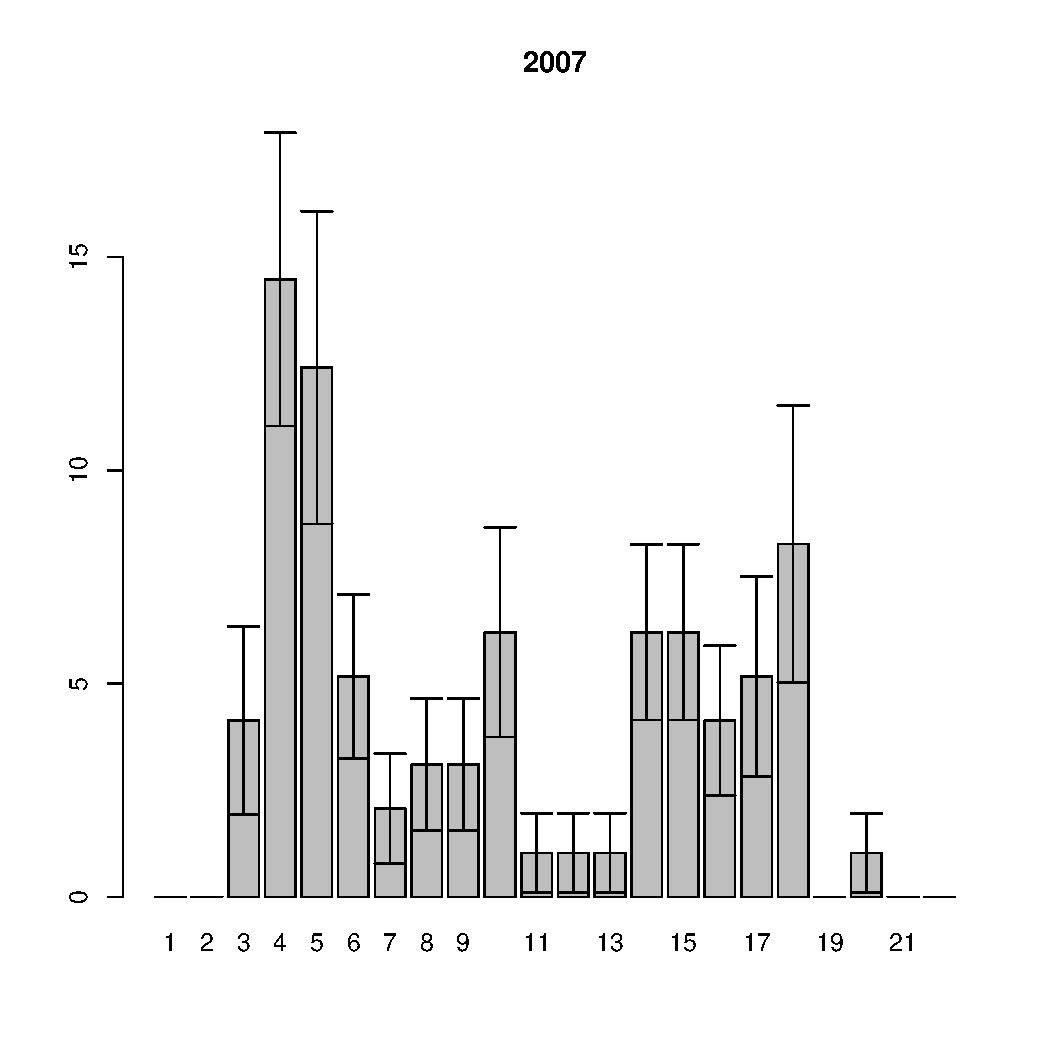
\includegraphics[width=55mm]{../Barenc_Sea/Yarnyshnaya/middle_2007_.pdf}
	\end{center}
	\end{minipage}
	%\smallskip
	\begin{minipage}[b]{.46\linewidth}

	\begin{center}
	{\footnotesize Ярнышная, НГЛ}
	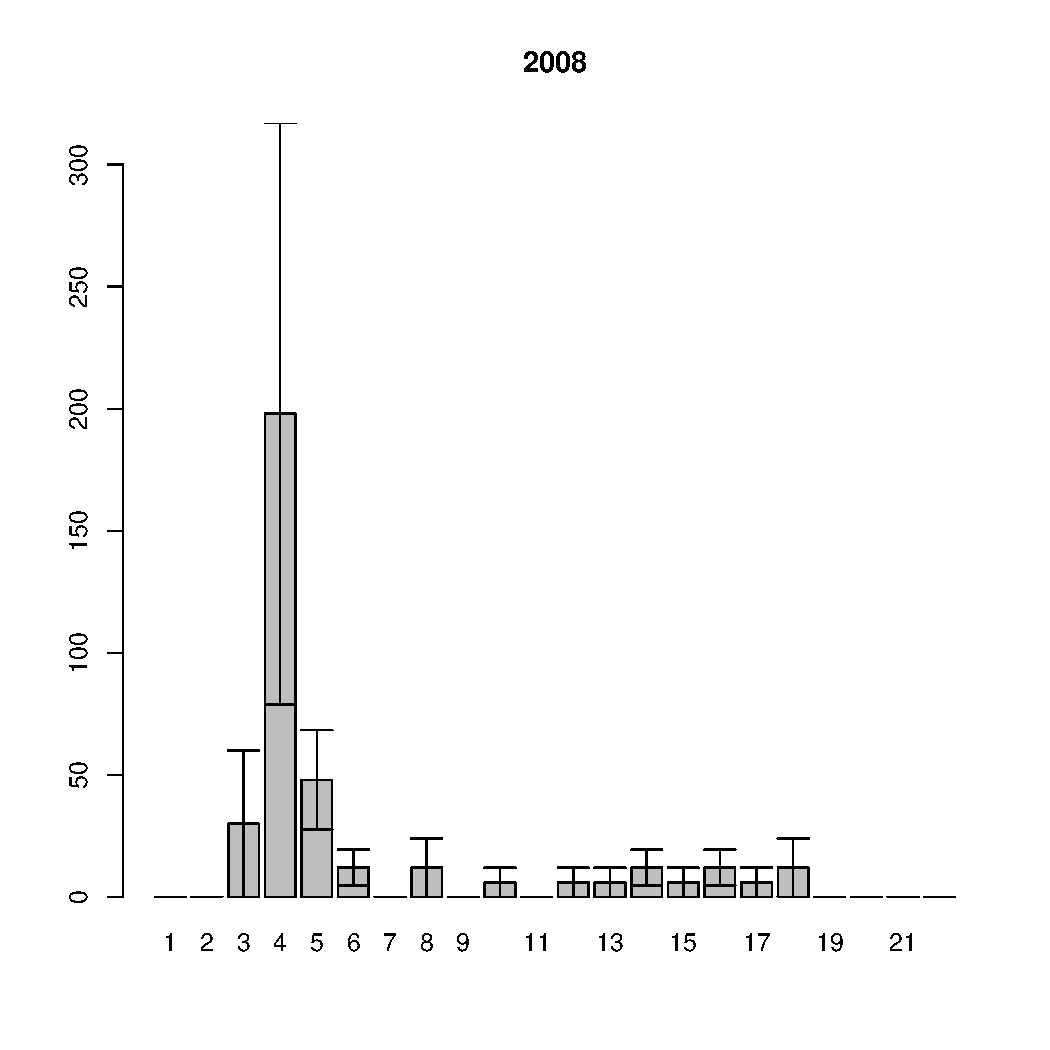
\includegraphics[width=55mm]{../Barenc_Sea/Yarnyshnaya/low_2008_.pdf}
	\end{center}
	\end{minipage}
	%	
	\hfil %Это пружинка отодвигающая рисунки друг от друга
	%
	\begin{minipage}[b]{.46\linewidth}
	\begin{center}	
	{\footnotesize Ивановская, ВСЛ}
	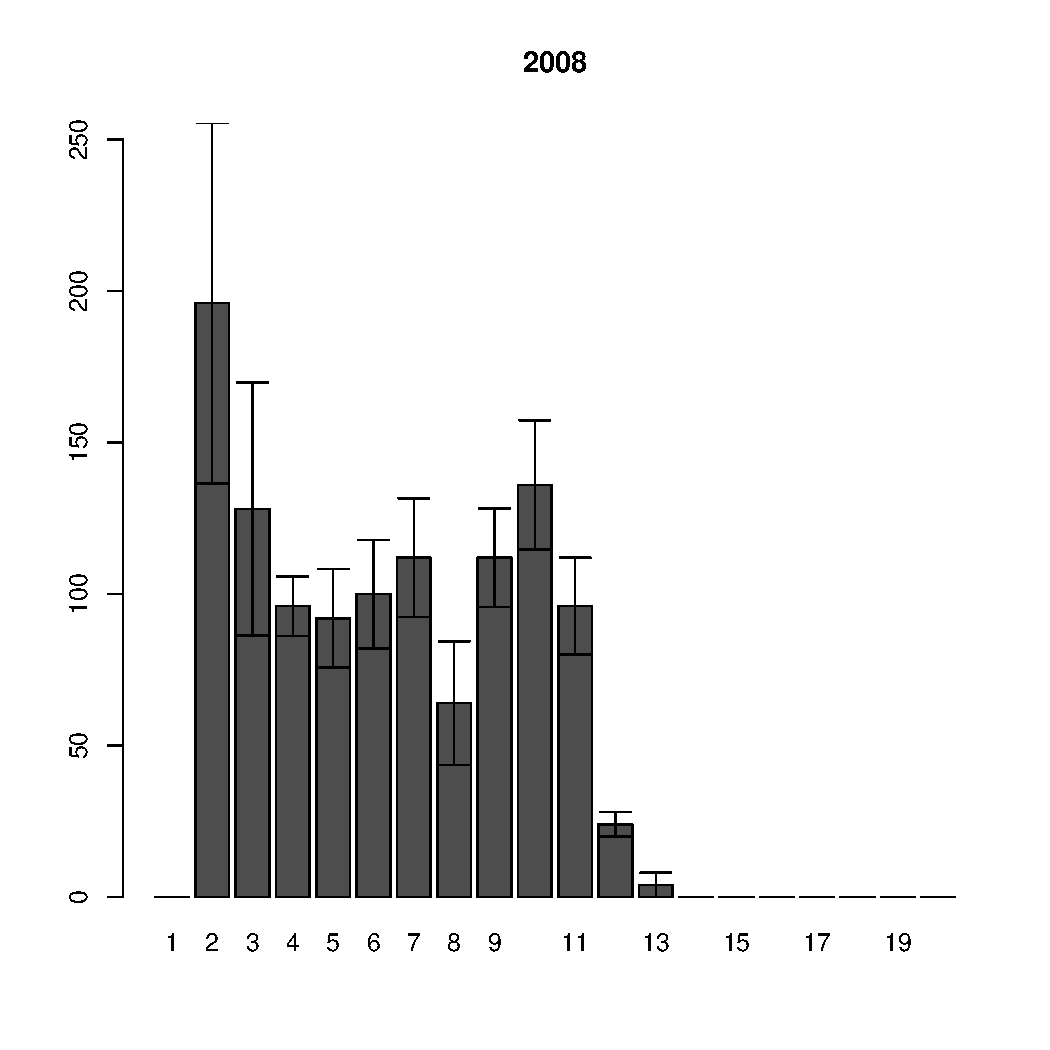
\includegraphics[width=55mm]{../Barenc_Sea/Ivanovskaya/sizestr2008.pdf}
	\end{center}
	\end{minipage}
	%\smallskip
	\begin{minipage}[b]{.46\linewidth}
	\begin{center}
	{\footnotesize Шельпино, ВГЛ}
	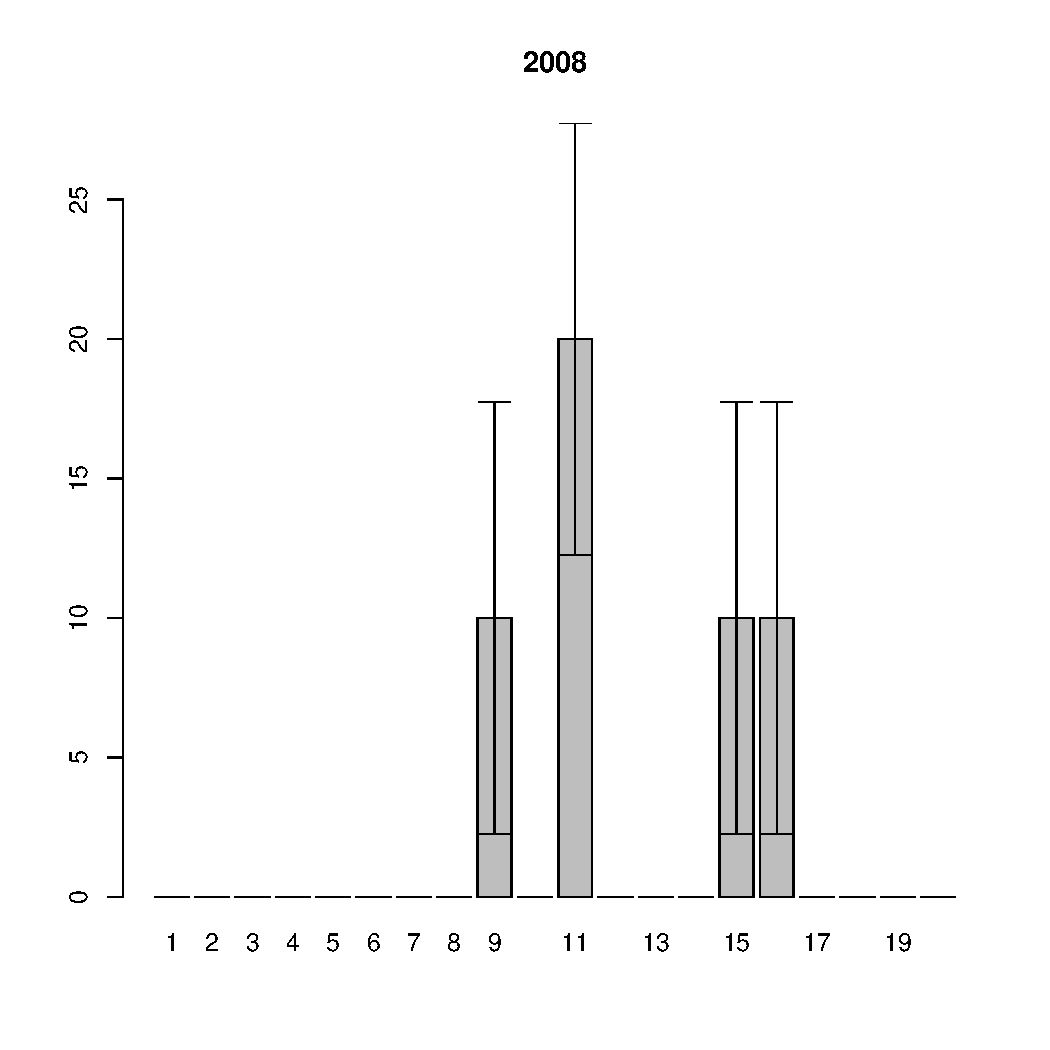
\includegraphics[width=55mm]{../Barenc_Sea/Shel'pino/high_2008_.pdf}
	\end{center}
	\end{minipage}
	%
	\hfil %Это пружинка отодвигающая рисунки друг от друга
	%
	\begin{minipage}[b]{.46\linewidth}
	\begin{center}
	{\footnotesize Шельпино, СГЛ}
	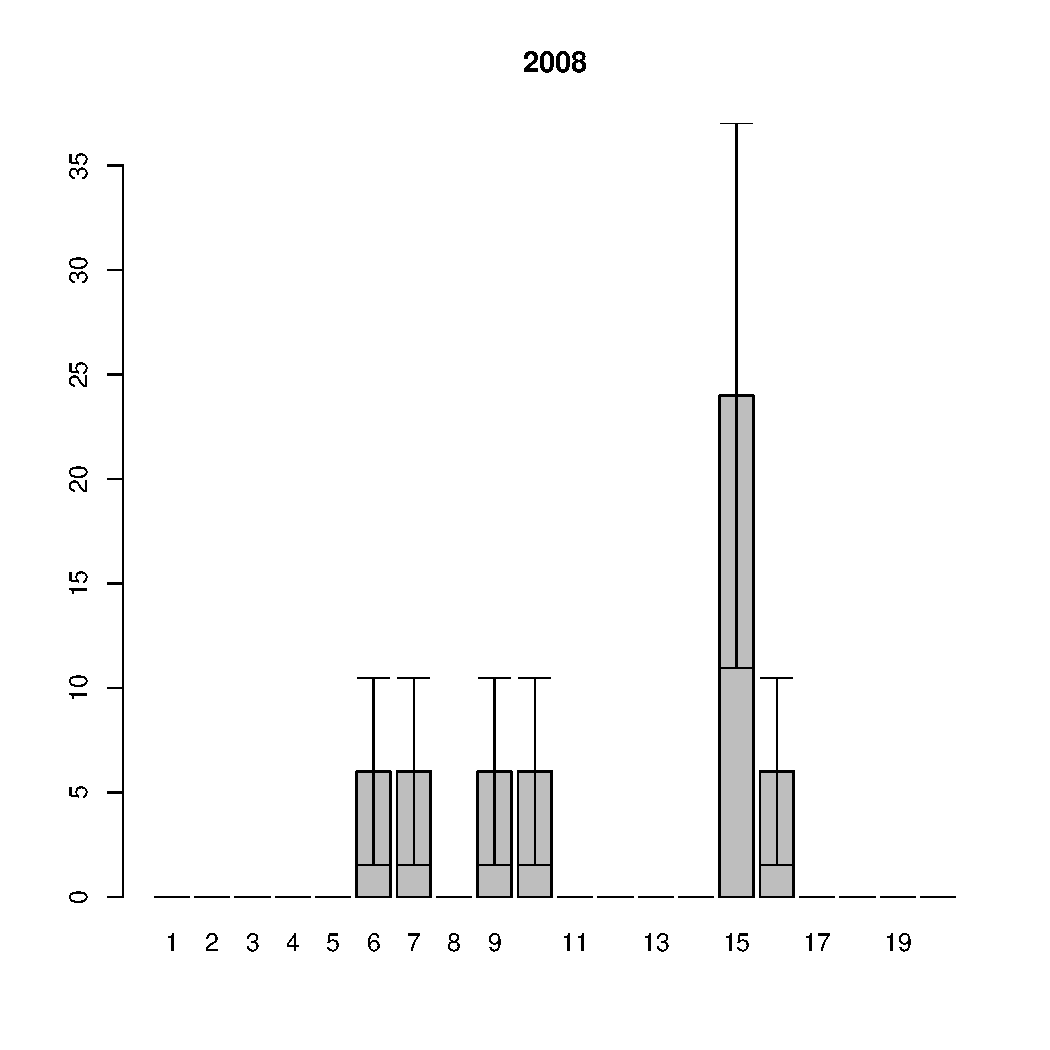
\includegraphics[width=55mm]{../Barenc_Sea/Shel'pino/middle_2008_.pdf}
	\end{center}
	\end{minipage}
	%\smallskip
\begin{center}
Рис. \ref{ris:Barents_sizestr} (продолжение). Размерная структура {\it Macoma balthica} в поселениях Мурманского побережья Баренцева моря
\end{center}
\end{figure}

%%%%%%%%%%%%%%%%%%
% Дальний пляж
	\begin{figure}[hp]

	\begin{minipage}[b]{.3\linewidth}
	\begin{center}
	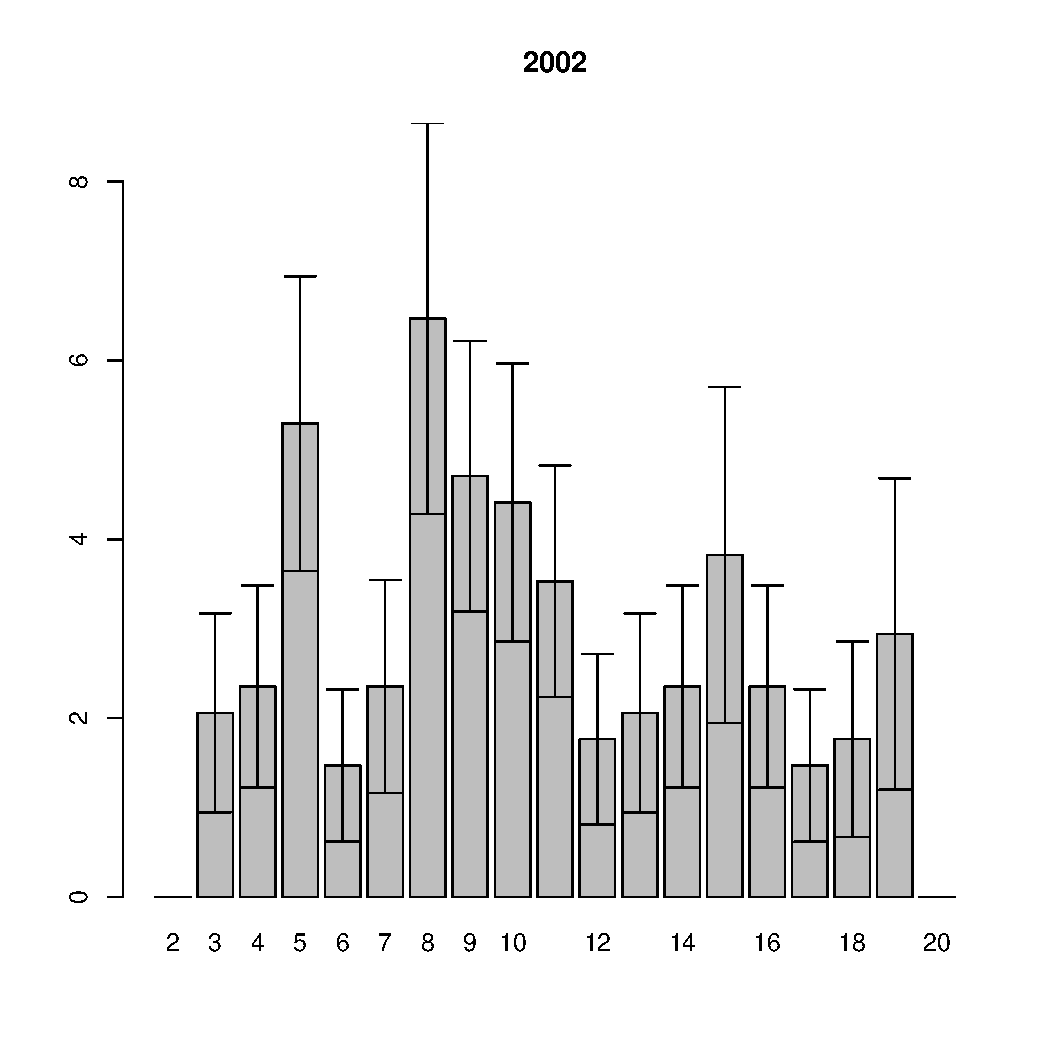
\includegraphics[width=60mm]{../Barenc_Sea/Dalnezeleneckaya/DZ2_2002_.pdf}	
	\end{center}
	\end{minipage}
	%
	\hfil %Это пружинка отодвигающая рисунки друг от друга
	%
	\begin{minipage}[b]{.3\linewidth}
	\begin{center}
	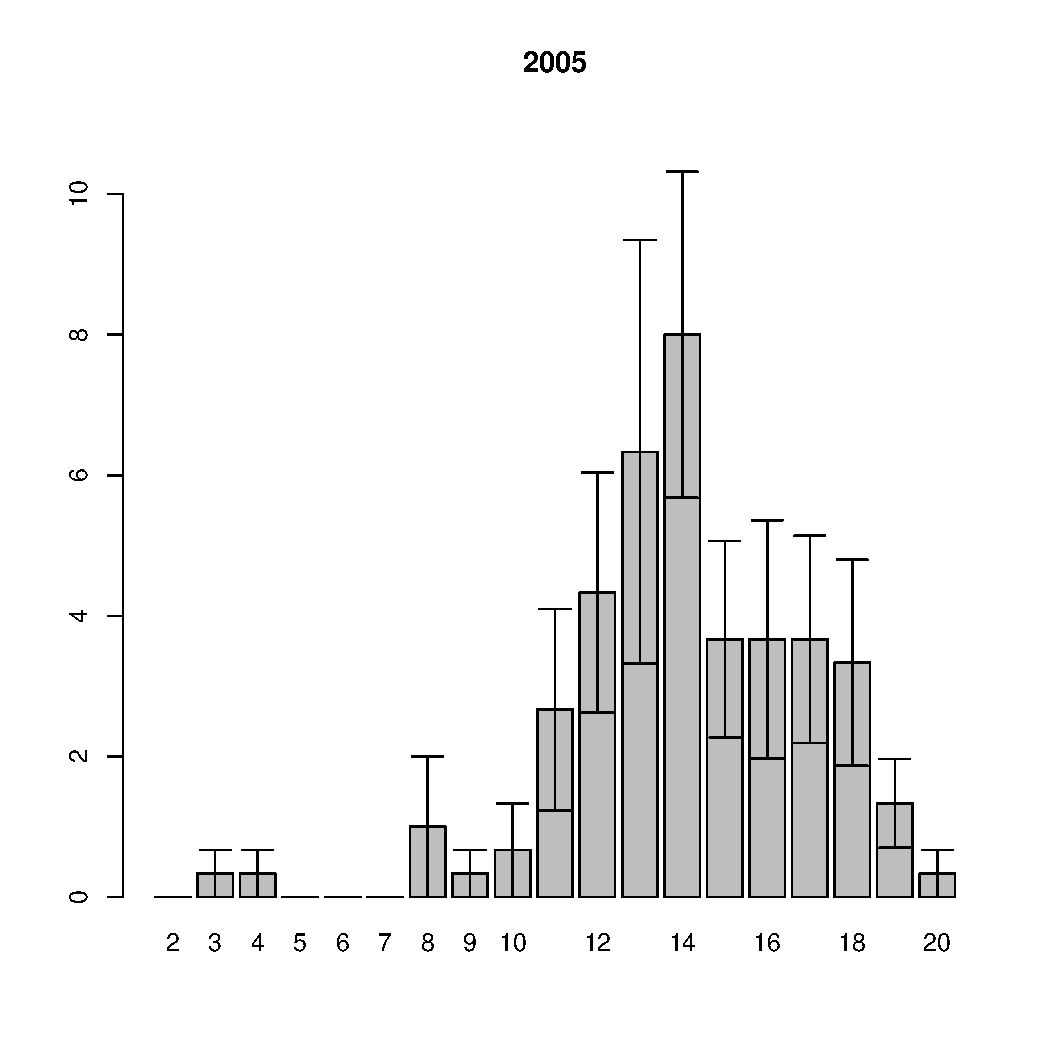
\includegraphics[width=60mm]{../Barenc_Sea/Dalnezeleneckaya/DZ2_2005_.pdf}
	\end{center}
	\end{minipage}
	%	
	\hfill
	%
	\begin{minipage}[b]{.3\linewidth}
	\begin{center}
	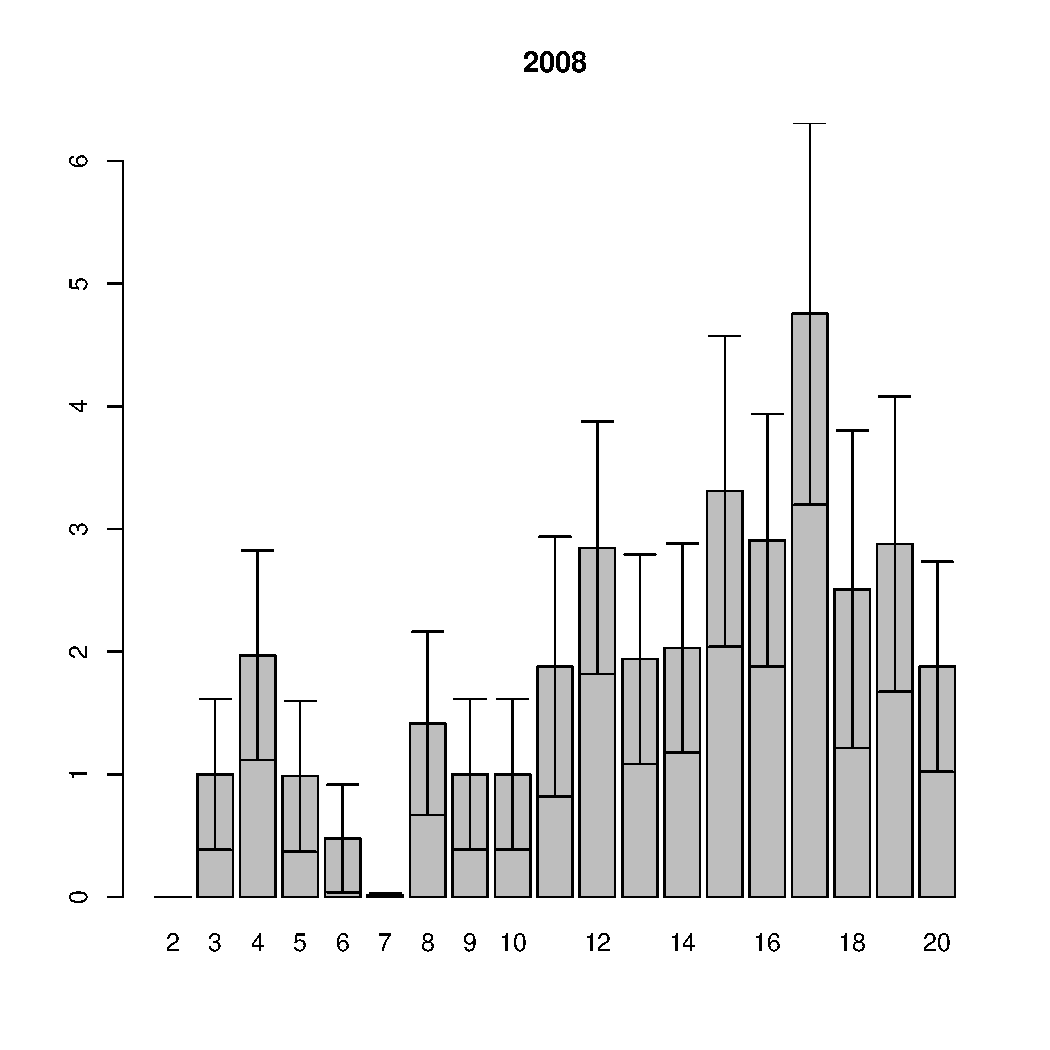
\includegraphics[width=60mm]{../Barenc_Sea/Dalnezeleneckaya/DZ2_2008_.pdf}
	\end{center}
	\end{minipage}
	%
	%
	\begin{minipage}[b]{.3\linewidth}
	\begin{center}
	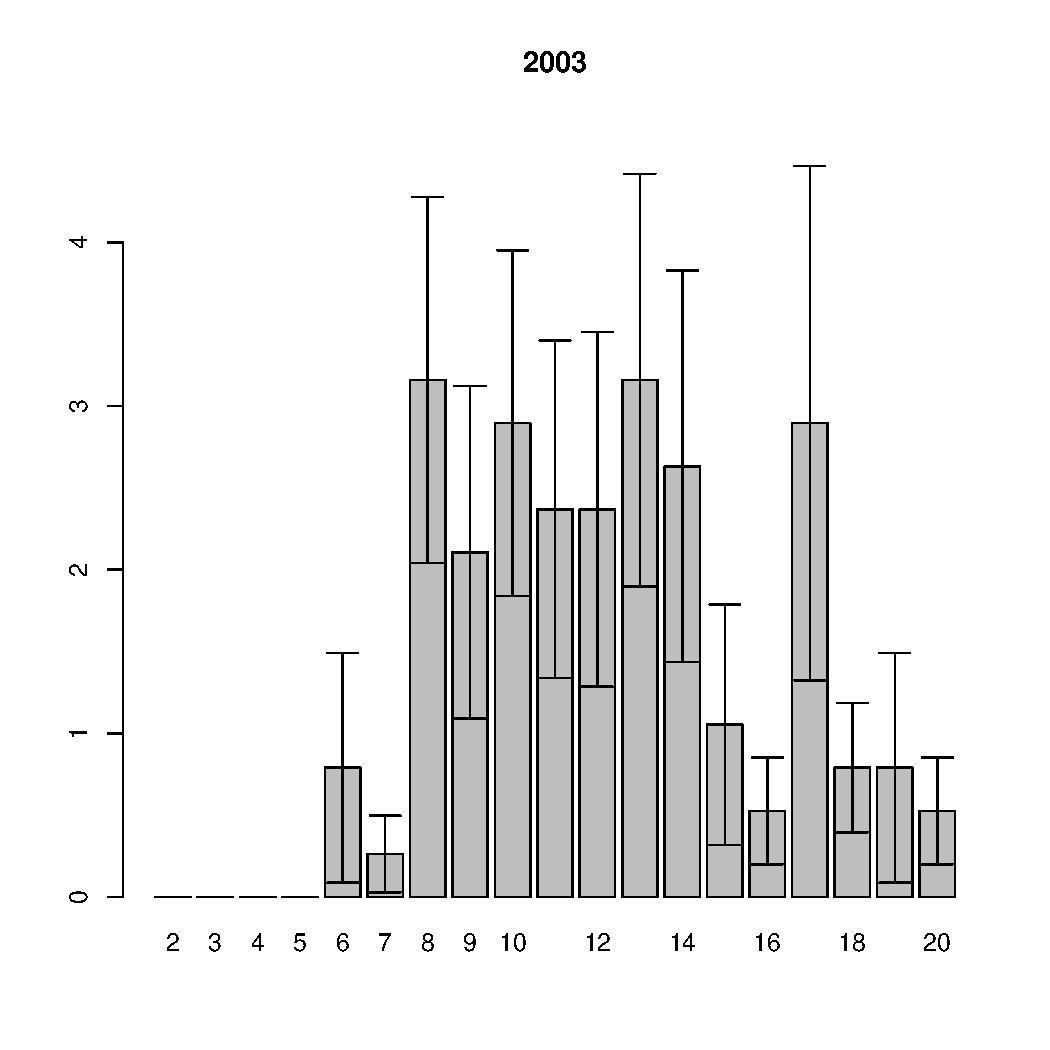
\includegraphics[width=60mm]{../Barenc_Sea/Dalnezeleneckaya/DZ2_2003_.pdf}
	\end{center}
	\end{minipage}
	%
	\hfill
	%
	\begin{minipage}[b]{.3\linewidth}
	\begin{center}
	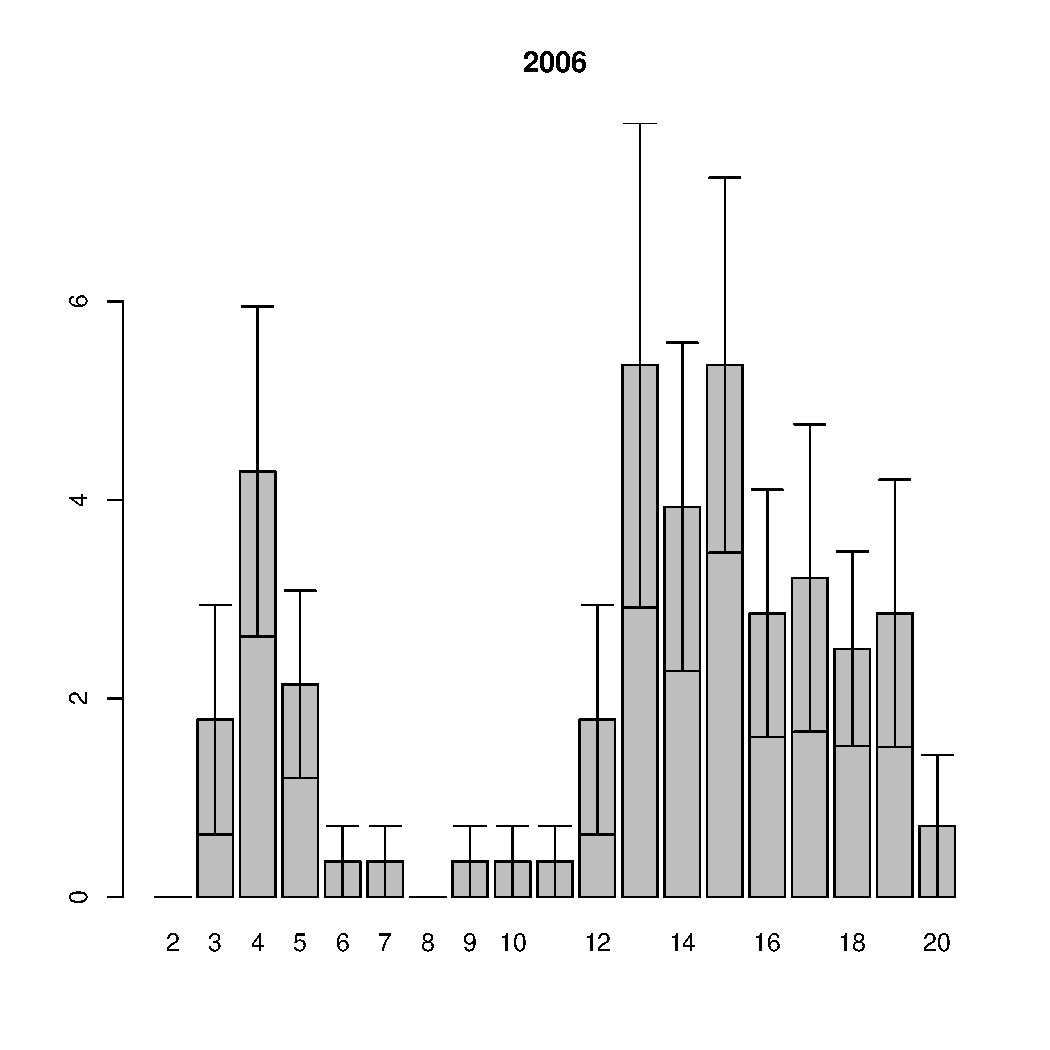
\includegraphics[width=60mm]{../Barenc_Sea/Dalnezeleneckaya/DZ2_2006_.pdf}
	\end{center}
	\end{minipage}
	%
	\hfill
	%
	\begin{minipage}[b]{.3\linewidth}
	\begin{center}
	
	\end{center}
	\end{minipage}
	%
	%
	\begin{minipage}[b]{.3\linewidth}
	\begin{center}
	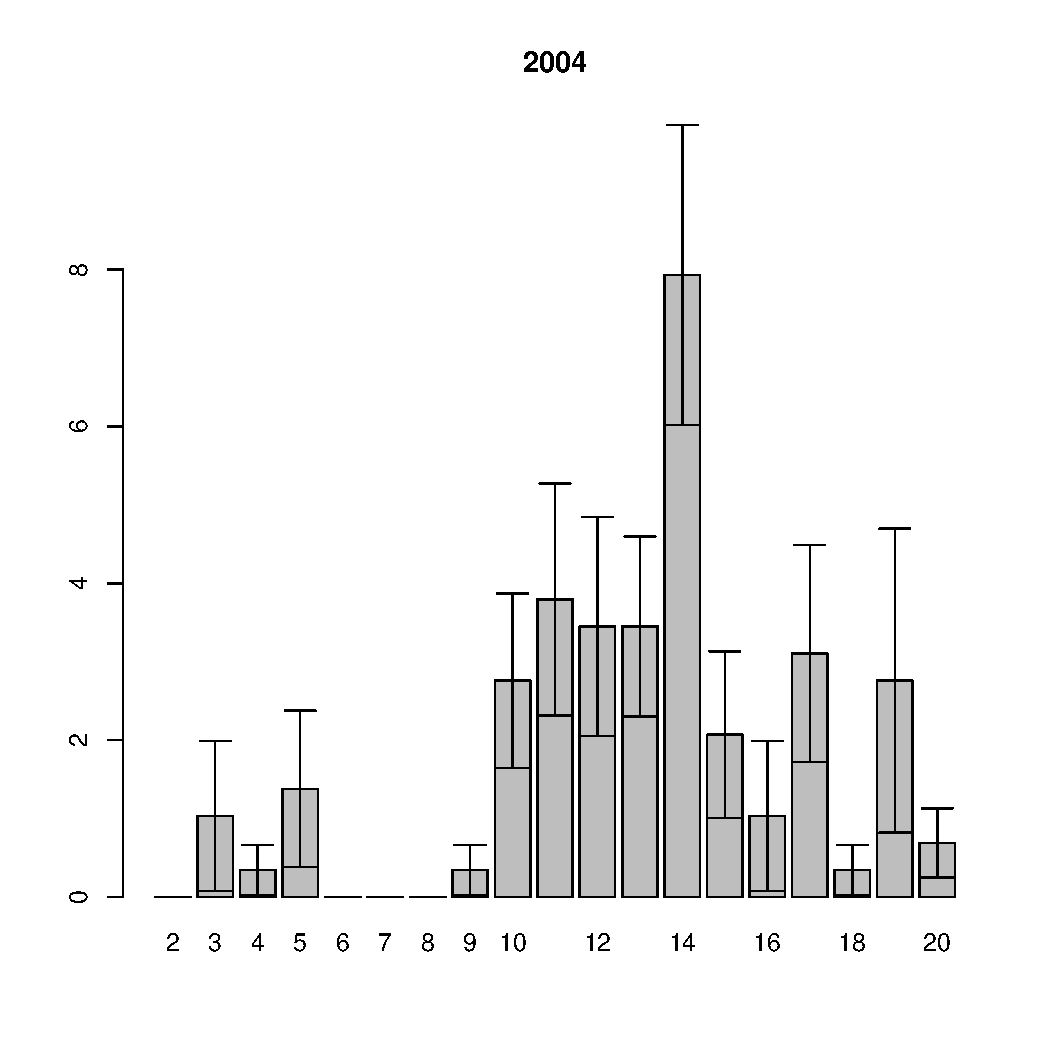
\includegraphics[width=60mm]{../Barenc_Sea/Dalnezeleneckaya/DZ2_2004_.pdf}
	\end{center}
	\end{minipage}	
	%
	\hfill
	%
	\begin{minipage}[b]{.3\linewidth}
	\begin{center}
	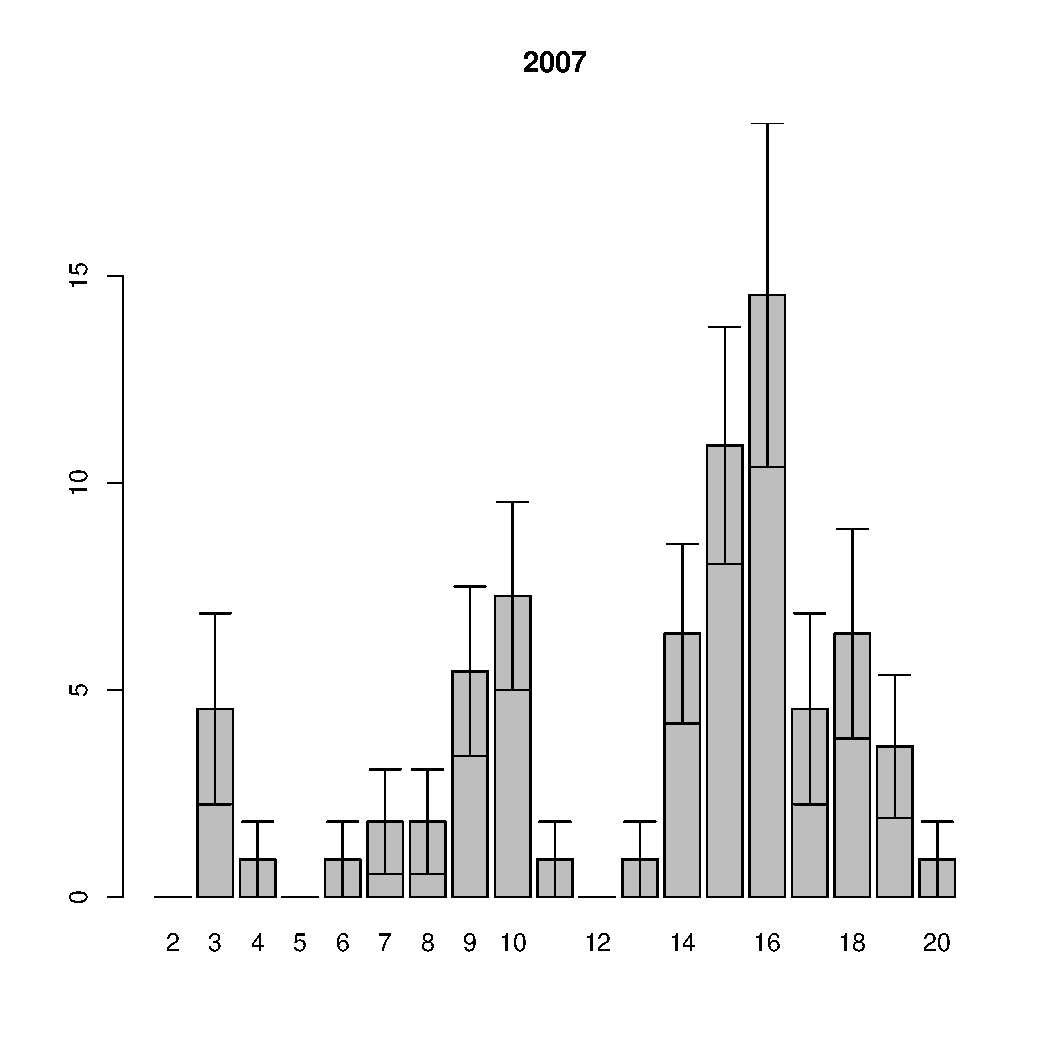
\includegraphics[width=60mm]{../Barenc_Sea/Dalnezeleneckaya/DZ2_2007_.pdf}
	\end{center}
	\end{minipage}
	%
	\hfill
	%
	\begin{minipage}[b]{.3\linewidth}
	\begin{center}

	\end{center}
	\end{minipage}

\caption{Размерная структура {\it Macoma balthica} на Дальнем пляже губы Дальнезеленецкая}
\label{ris:size_str_DZ}
\end{figure}
